\documentclass{article}
\usepackage[utf8]{inputenc}
\usepackage{amsmath,amssymb}
\usepackage{graphicx}
\usepackage{float}
\usepackage{subcaption}
\usepackage{geometry}
\geometry{
    a4paper,
    total={170mm,257mm},
    left=20mm,
    right=20mm,
    top=20mm,
}
\usepackage{listings} % code listings
\lstset{framextopmargin=0pt,frame=lines}
\lstset{
    language=Matlab,
    basicstyle=\footnotesize\ttfamily,
    breaklines=true,
    tabsize=4,
    keepspaces=true,
    columns=flexible,
    % backgroundcolor=\color[gray]{0.9},
    frame=single,
    breaklines=true,%
    morekeywords={matlab2tikz},
    keywordstyle=\color{blue},%
    morekeywords=[2]{1}, keywordstyle=[2]{\color{black}},
    identifierstyle=\color{black},%
    stringstyle=\color{mylilas},
    commentstyle=\color{mygreen},%
    showstringspaces=false,%without this there will be a symbol in the places where there is a space
    numbers=left,
    numberstyle={\tiny \color{black}},% size of the numbers
    numbersep=9pt, % this defines how far the numbers are from the text
    emph=[1]{for,end,break},emphstyle=[1]\color{red}, %some words to emphasise
    %emph=[2]{word1,word2}, emphstyle=[2]{style},
}
\usepackage{color} %red, green, blue, yellow, cyan, magenta, black, white
\definecolor{mygreen}{RGB}{28,172,0} % color values Red, Green, Blue
\definecolor{mylilas}{RGB}{170,55,241}

\usepackage{siunitx}
\newcommand{\e}[1]{\times 10^{#1}} % nicer scientific notation

\title{ENV-541 Sensor Orientation\\Lab 5 - Inertial Navigation in 2D / Realistic Signal}
\author{Michael Spieler}
\date{November 2, 2018}

\begin{document}

\maketitle

\section*{Stochastic error values}

Table \ref{tab:err_val} lists the parameters for the different stochastic error sources used in this lab.
\begin{table}[h]
\centering
\begin{tabular}{lllll}
Error type & Notation & Value & Units & Note \\
\hline
\textbf{Gyro} bias (random constant) & $b_G$ & $4.848\e{-5}$ & $\si{\radian/\second}$ & $1\sigma$ \\
\textbf{Gyro} correlation noise (1st order Gauss-Markov) & $\sigma_{G^{PSD}_{GM1}}$ & $8.727\e{-5}$ & $\si{\radian/\second/\sqrt{\hertz}}$ & PSD level \\
& $1/\beta_G$ & $100$ & $\si{\second}$ & correlation time \\
\textbf{Gyro} random walk (white noise) & $\sigma_{G^{PSD}_{WN}}$  & $2.909\e{-4}$ & $\si{\radian/\second/sample}$ & PSD level \\
% \hline
\textbf{Accel} bias (random constant) & $b_A$  & $9.807 \e{-3}$ & $\si{\meter/\second^2}$ & $1\sigma$ \\
\textbf{Accel} noise (white)  & $\sigma_{G^{PSD}_{WN}}$ & $4.904\e{-3}$ & $\si{\meter/\second^2/sample}$ & PSD level
\end{tabular}
\caption{Stochastic error values in SI units.}
\label{tab:err_val}
\end{table}

\section*{Error plots}

The 2D strapdown inertial navigatin example along a circle was simulated with a 100Hz sample frequency.
The trapezoidal integration method was used for the state estimation.

\subsection*{Individual error sources}
In a first step the experiment was performed for each error source individally.
Maximal (absolute) estimation errors along the trajectory are summarized in table \ref{tab:err_result}.

\begin{table}[h]
\centering
\begin{tabular}{llll}
Error  & Azimuth error & Velocity error & Position error \\
\hline
\textbf{Gyro} Const. random bias & $5.756\e{-1}$ deg & $1.580\e{-1} \si{m/s}$ & $1.007\e{+1} \si{m}$ \\
\textbf{Gyro} 1st order Gauss-Markov & $\mathbf{8.724\e{-1}}$ deg & $3.409\e{-1} \si{m/s}$ & $1.739\e{+1} \si{m}$ \\
\textbf{Gyro} White noise & $2.480\e{-2}$ deg & $9.535\e{-3} \si{m/s}$ & $1.290\e{+0} \si{m}$ \\
\hline
\textbf{Accel} Const. random bias & $2.328\e{-10}$ deg & $\mathbf{1.172\e{+0}} \si{m/s}$ & $\mathbf{1.172\e{+2}} \si{m}$ \\
\textbf{Accel} White noise & $2.328\e{-10}$ deg & $1.337\e{-2} \si{m/s}$ & $1.509\e{+0} \si{m}$ 
\end{tabular}
\caption{Estimation errors from different error sources}
\label{tab:err_result}
\end{table}


Figure \ref{fig:error_gyro} shows the estimation error evolution for each gyro error source as well as for all sources combined.

\begin{figure}[H]
    \centering
    \begin{subfigure}[t]{0.49\textwidth}
        \centering
        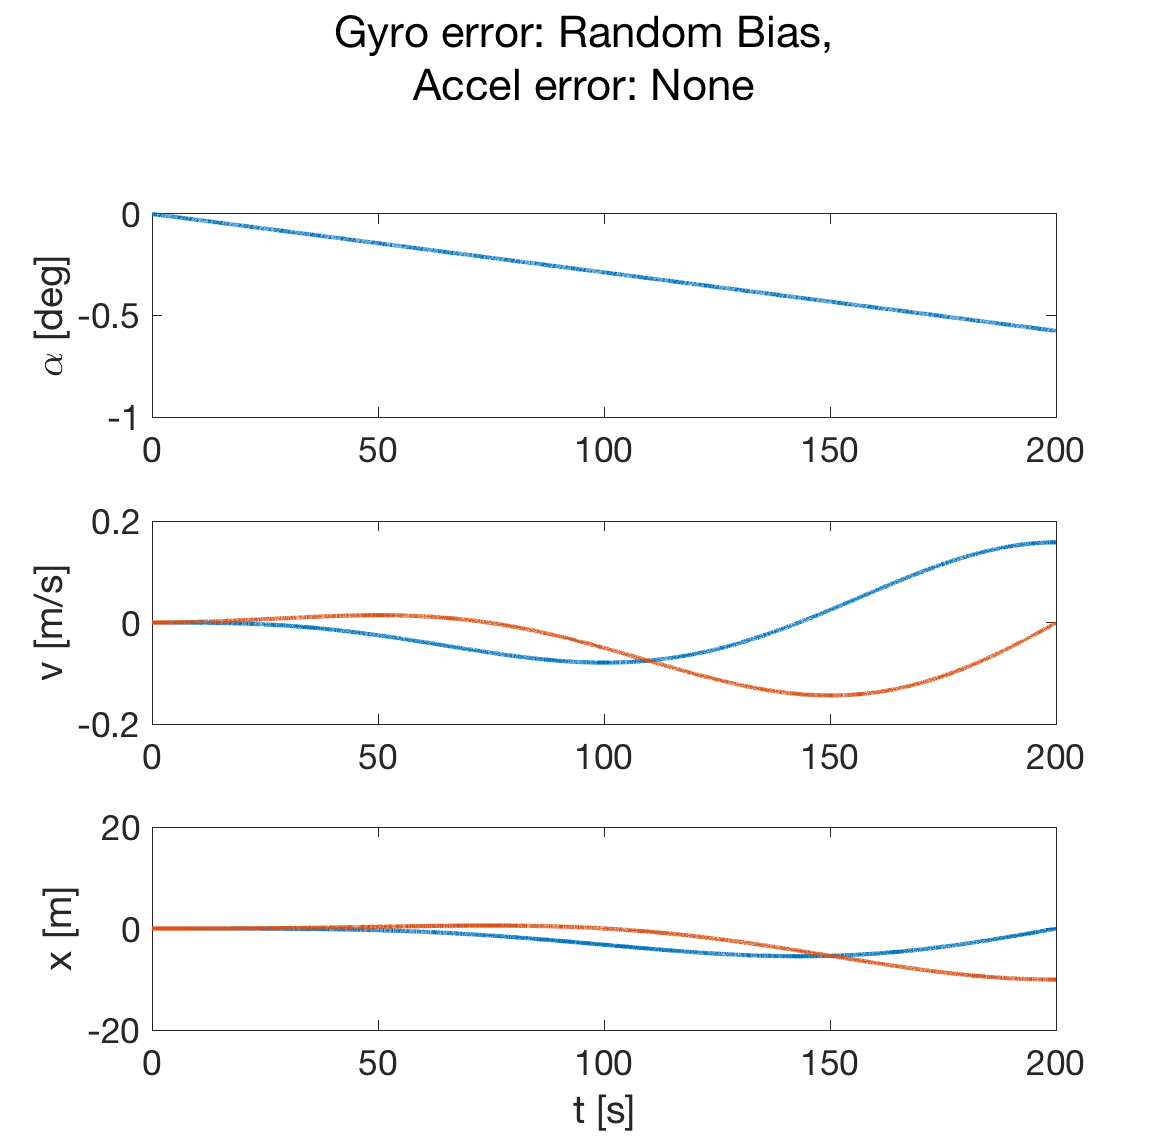
\includegraphics[width=\textwidth]{fig/gyro_bc}
        % \caption{}
    \end{subfigure}
    ~
    \begin{subfigure}[t]{0.49\textwidth}
        \centering
        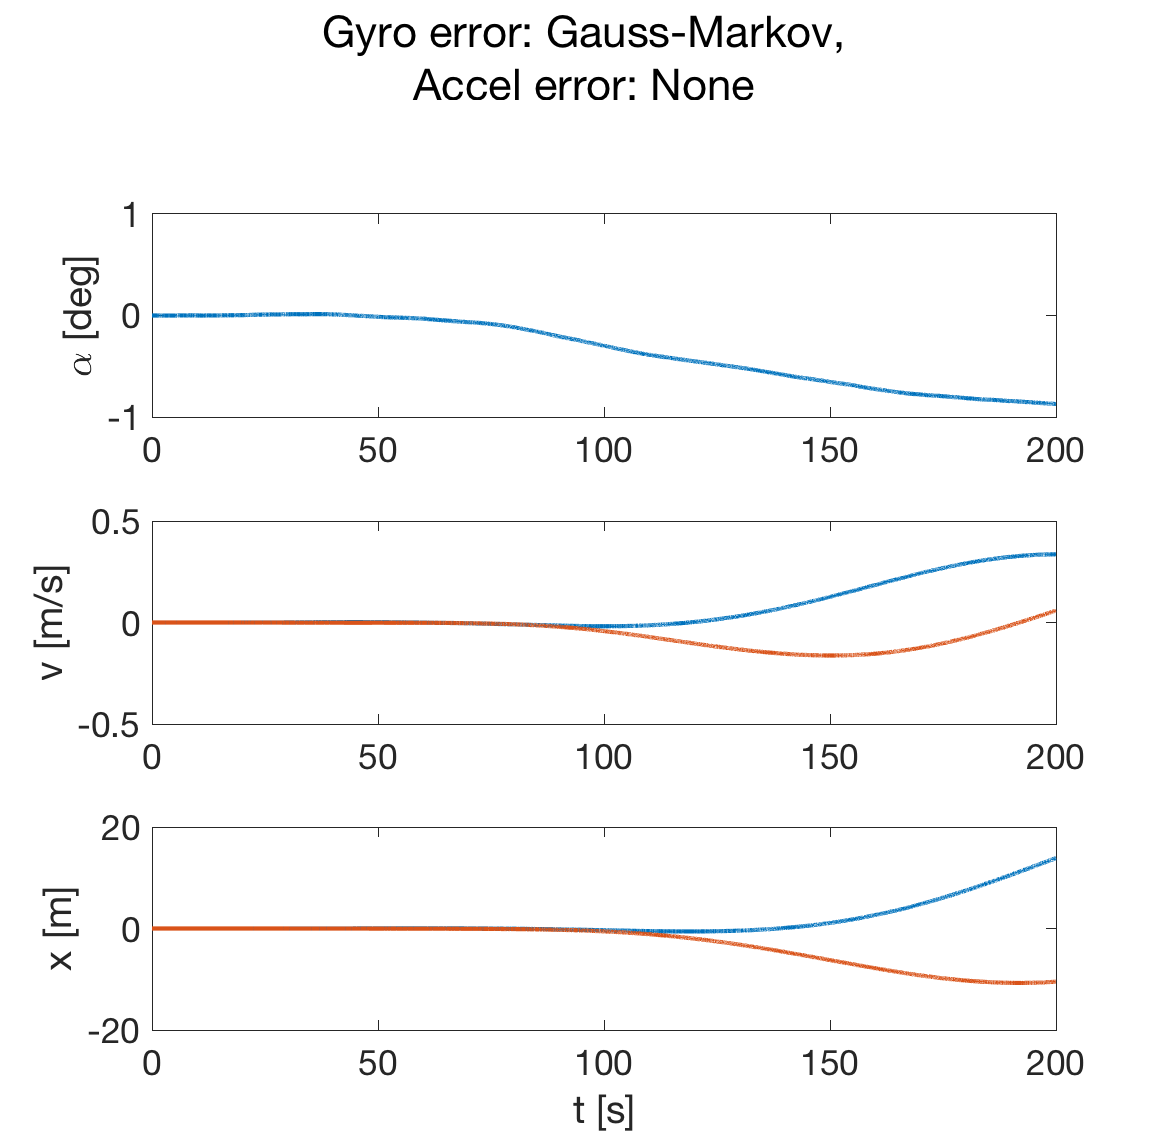
\includegraphics[width=\textwidth]{fig/gyro_gm}
        % \caption{}
    \end{subfigure}
    ~
    \begin{subfigure}[t]{0.49\textwidth}
        \centering
        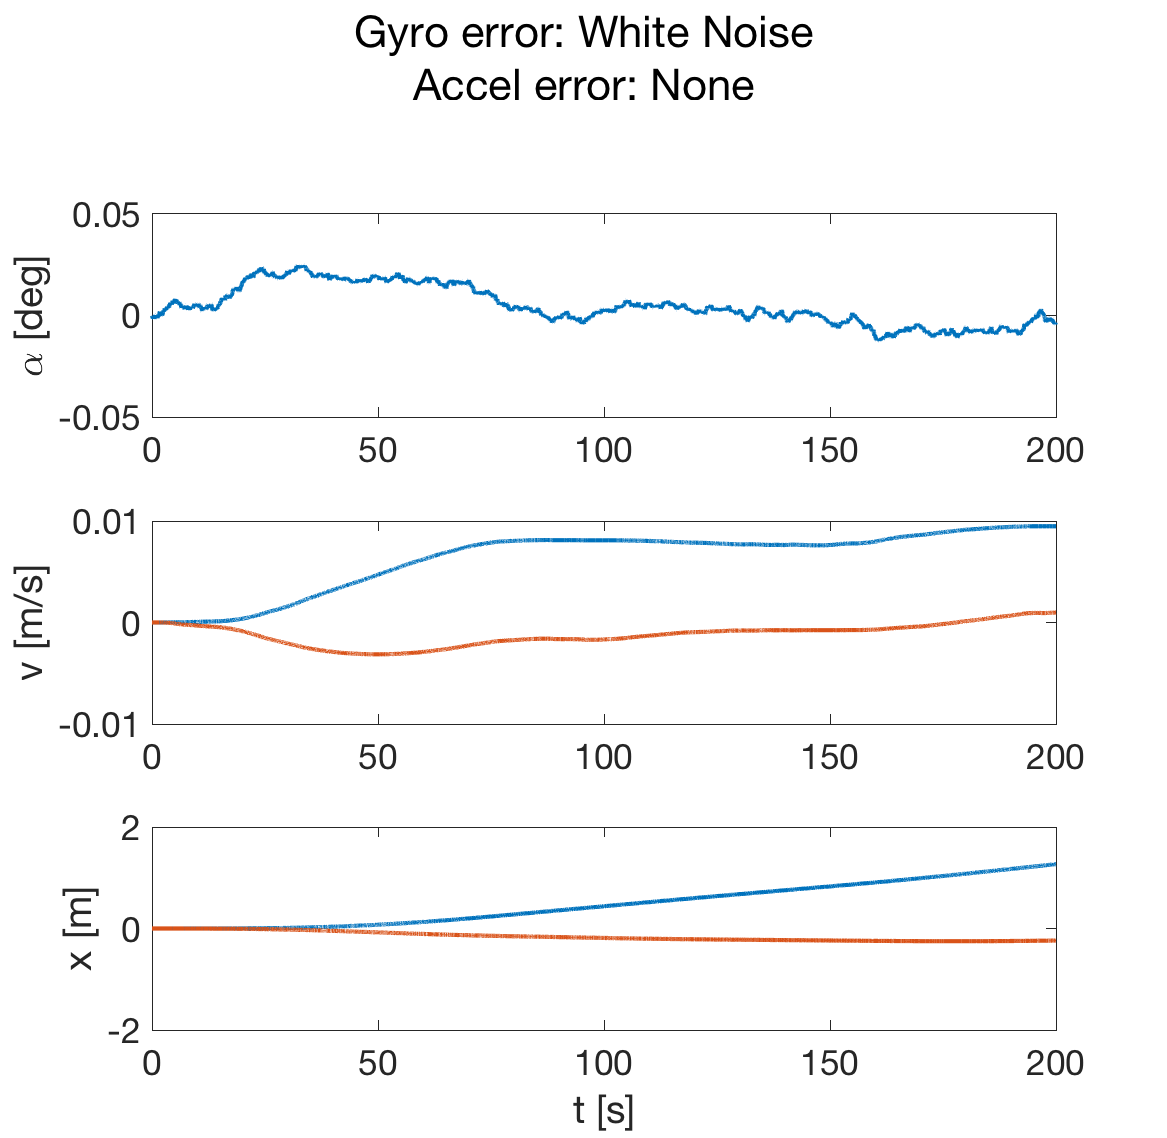
\includegraphics[width=\textwidth]{fig/gyro_wn}
        % \caption{}
    \end{subfigure}
    ~
    \begin{subfigure}[t]{0.49\textwidth}
        \centering
        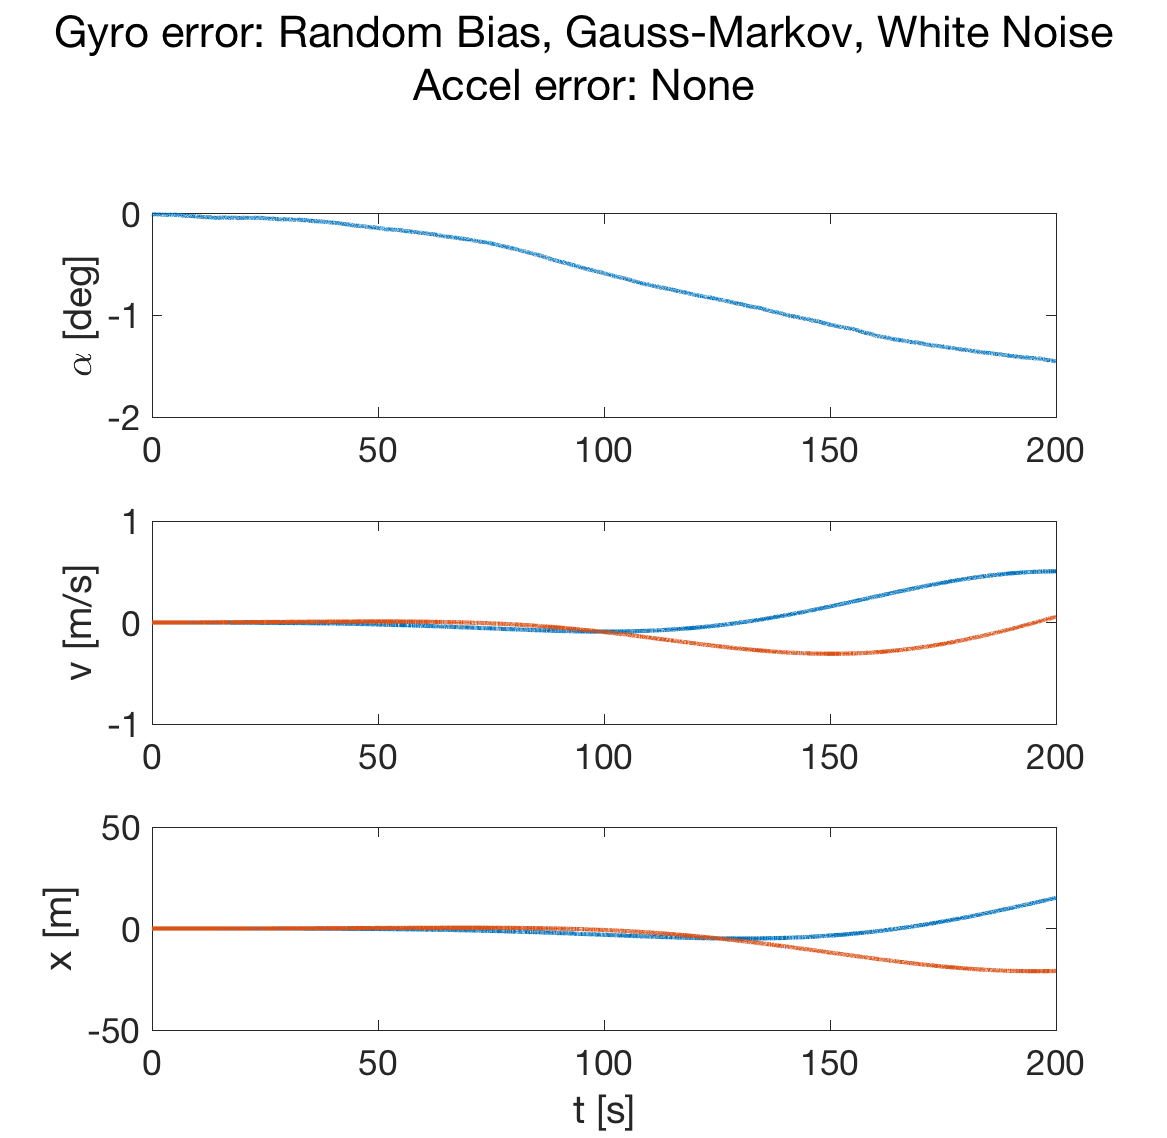
\includegraphics[width=\textwidth]{fig/gyro_all}
        % \caption{}
    \end{subfigure}
    \caption{Trajectory errors from gyro noise}
    \label{fig:error_gyro}
\end{figure}

Figure \ref{fig:error_accel} shows the estimation error evolution for the accelerometer
error sources of constant random bias and white noise as well as both combined.

\begin{figure}[H]
    \centering
    \begin{subfigure}[t]{0.49\textwidth}
        \centering
        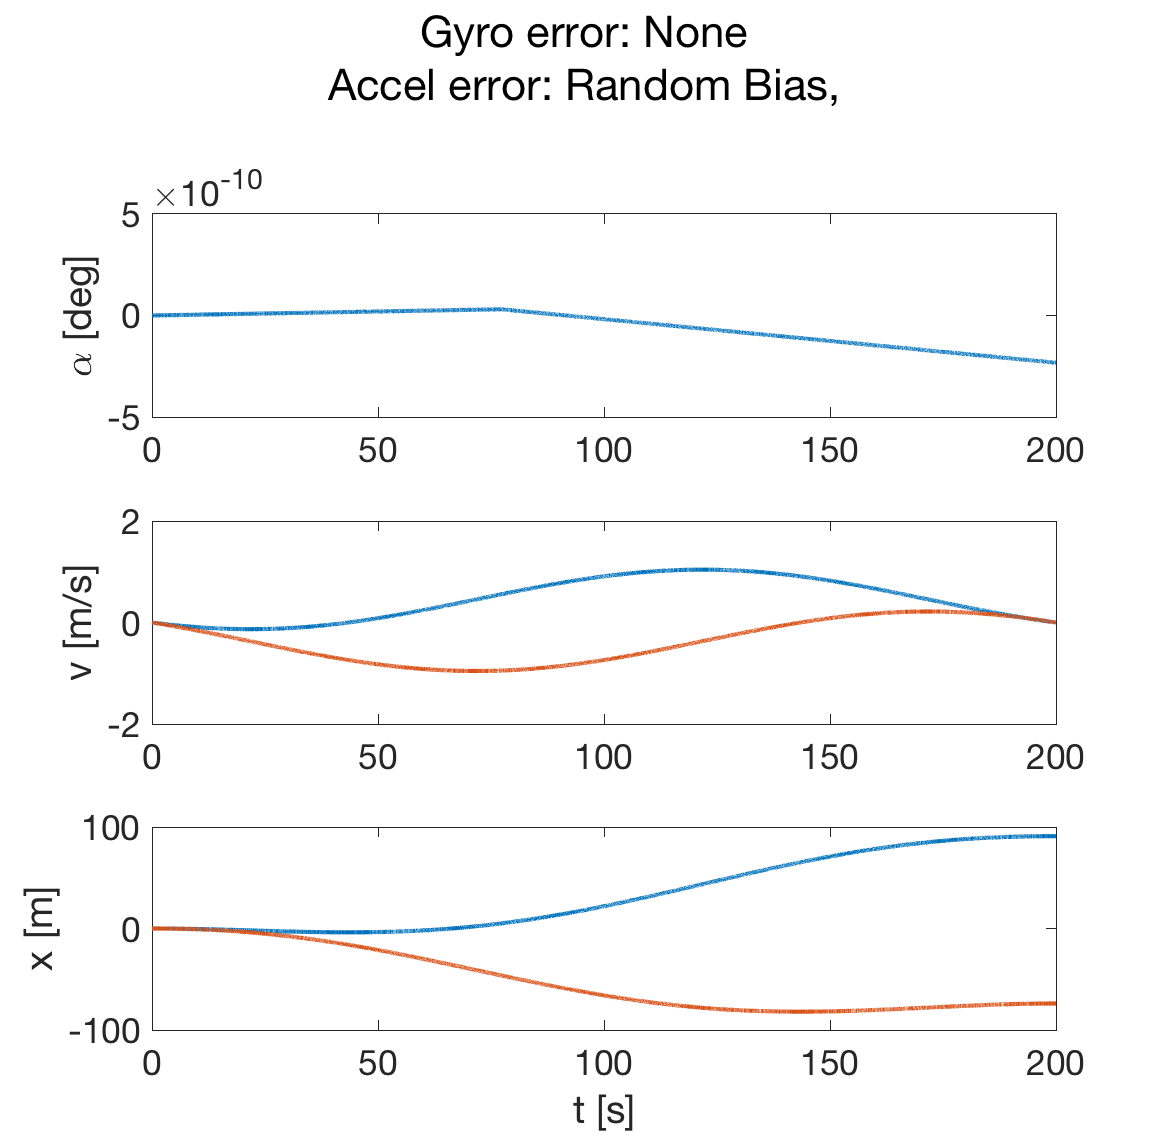
\includegraphics[width=\textwidth]{fig/accel_bc}
        \caption{}
    \end{subfigure}
    ~
    \begin{subfigure}[t]{0.49\textwidth}
        \centering
        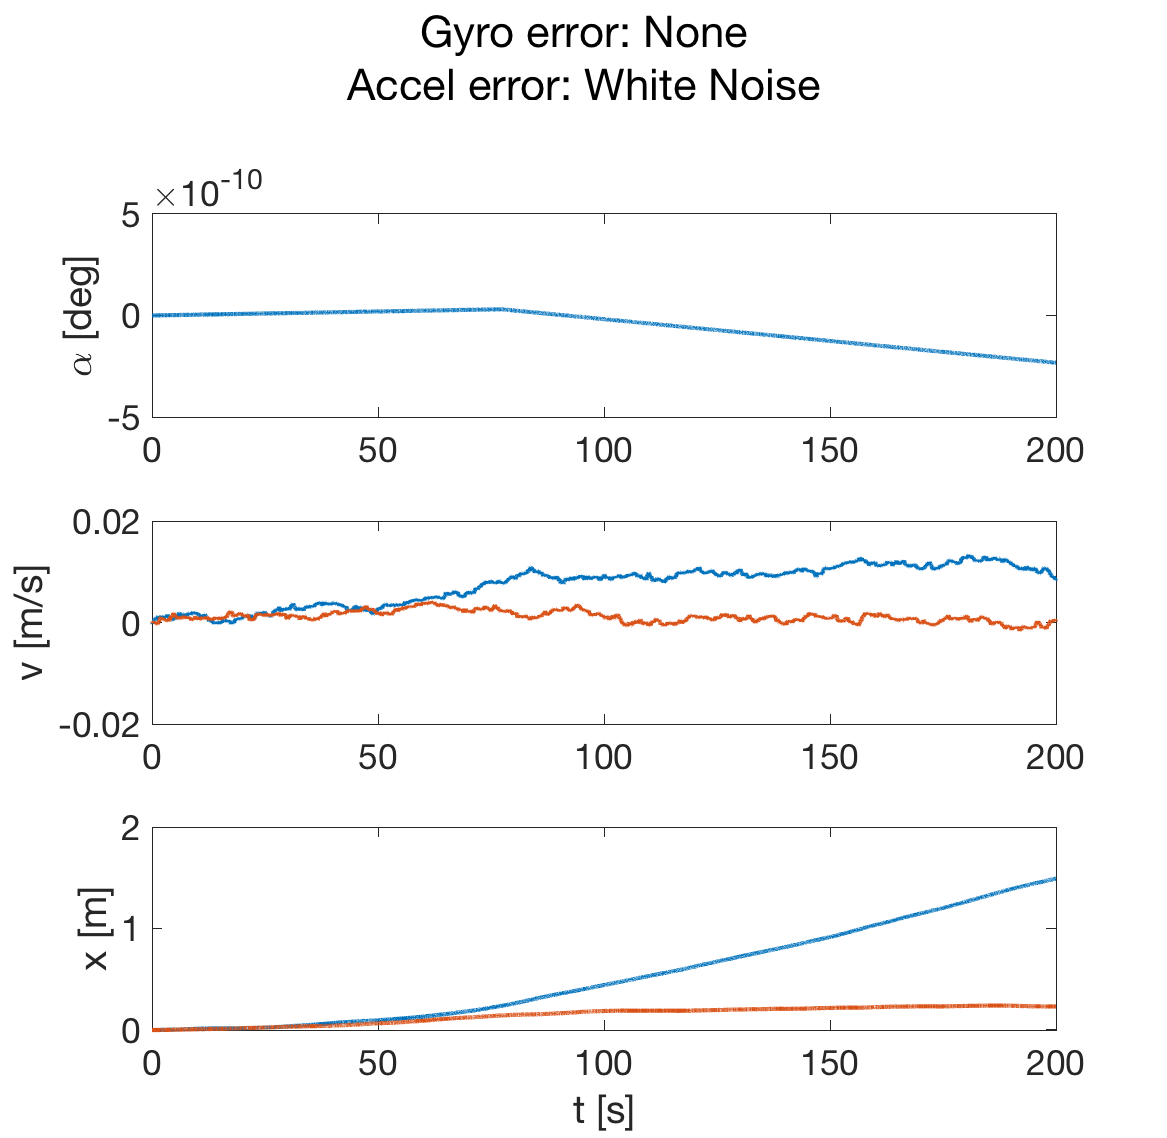
\includegraphics[width=\textwidth]{fig/accel_wn}
        \caption{}
    \end{subfigure}
    ~
    \begin{subfigure}[t]{0.49\textwidth}
        \centering
        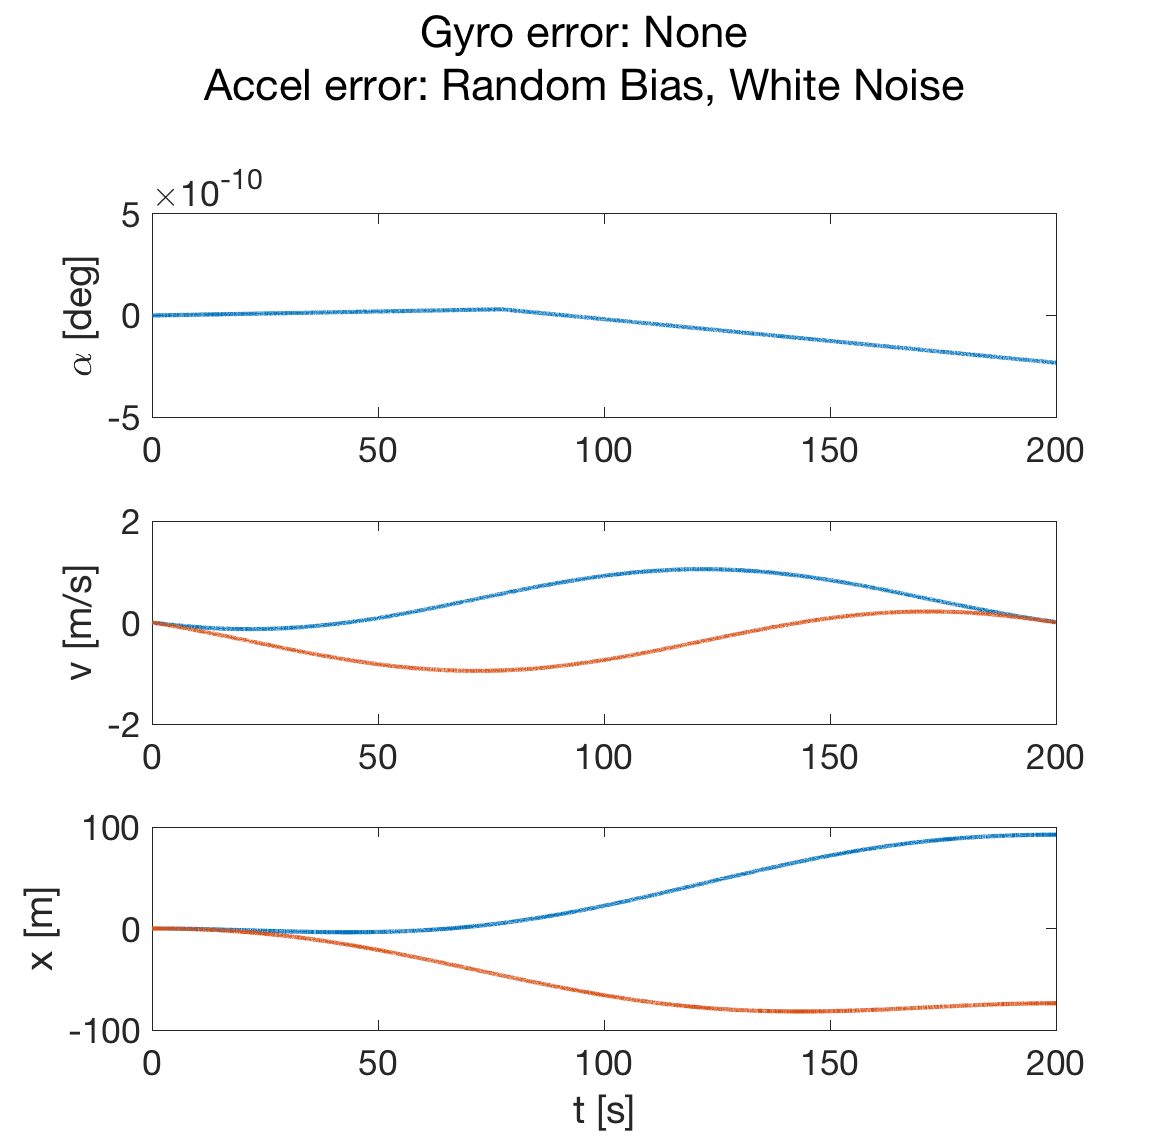
\includegraphics[width=\textwidth]{fig/accel_all}
        \caption{}
    \end{subfigure}
    \caption{Trajectory errors from accelerometer noise}
    \label{fig:error_accel}
\end{figure}

\subsection*{Combined error sources}

The estimation errors along the trajectory for the combined error sources are summarized in table \ref{tab:combined_err}.
Figure \ref{fig:error_all} shows the estimation error evolution for all error sources enabled as well as the resulting trajectory estimate.

\begin{table}[h]
\centering
\begin{tabular}{llll}
Error  & Azimuth error & Velocity error & Position error \\
\hline
Gyro all & $1.452\e{+0}$ deg & $5.076\e{-1} \si{m/s}$ & $2.577\e{+1} \si{m}$ \\
Accel all & $2.328\e{-10}$ deg & $1.179\e{+0} \si{m/s}$ & $1.182\e{+2} \si{m}$ \\
Gyro + Accel & $1.452\e{+0}$ deg & $1.188\e{+0} \si{m/s}$ & $1.439\e{+2} \si{m}$
\end{tabular}
\caption{Estimation errors with combined error sources.}
\label{tab:combined_err}
\end{table}

\begin{figure}[H]
    \centering
    \begin{subfigure}[t]{0.49\textwidth}
        \centering
        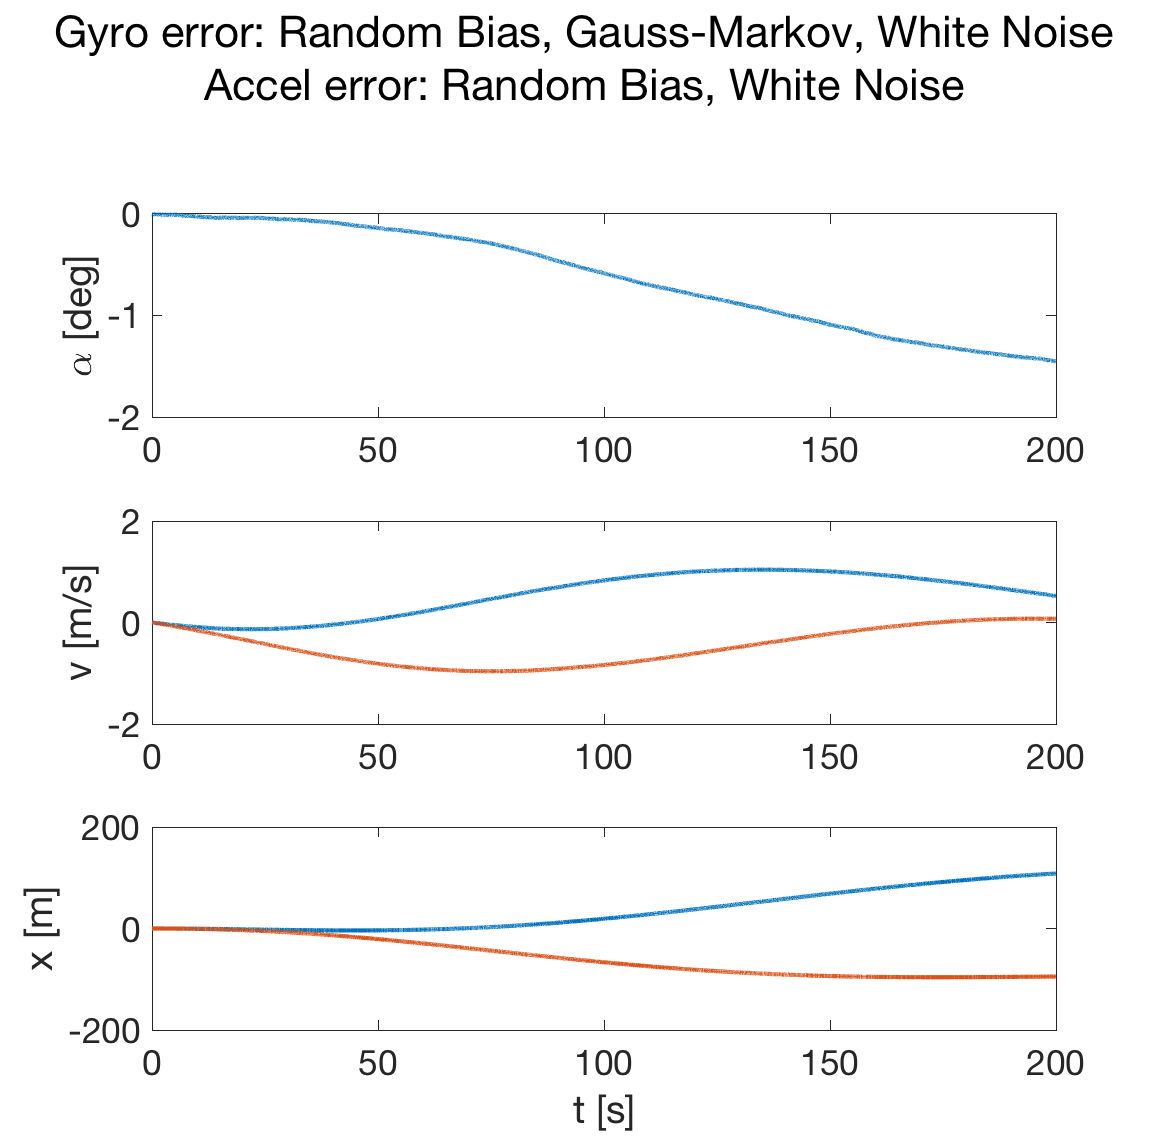
\includegraphics[width=\textwidth]{fig/all}
        \caption{Trajectory errors from all error sources.}
    \end{subfigure}
    ~
    \begin{subfigure}[t]{0.49\textwidth}
        \centering
        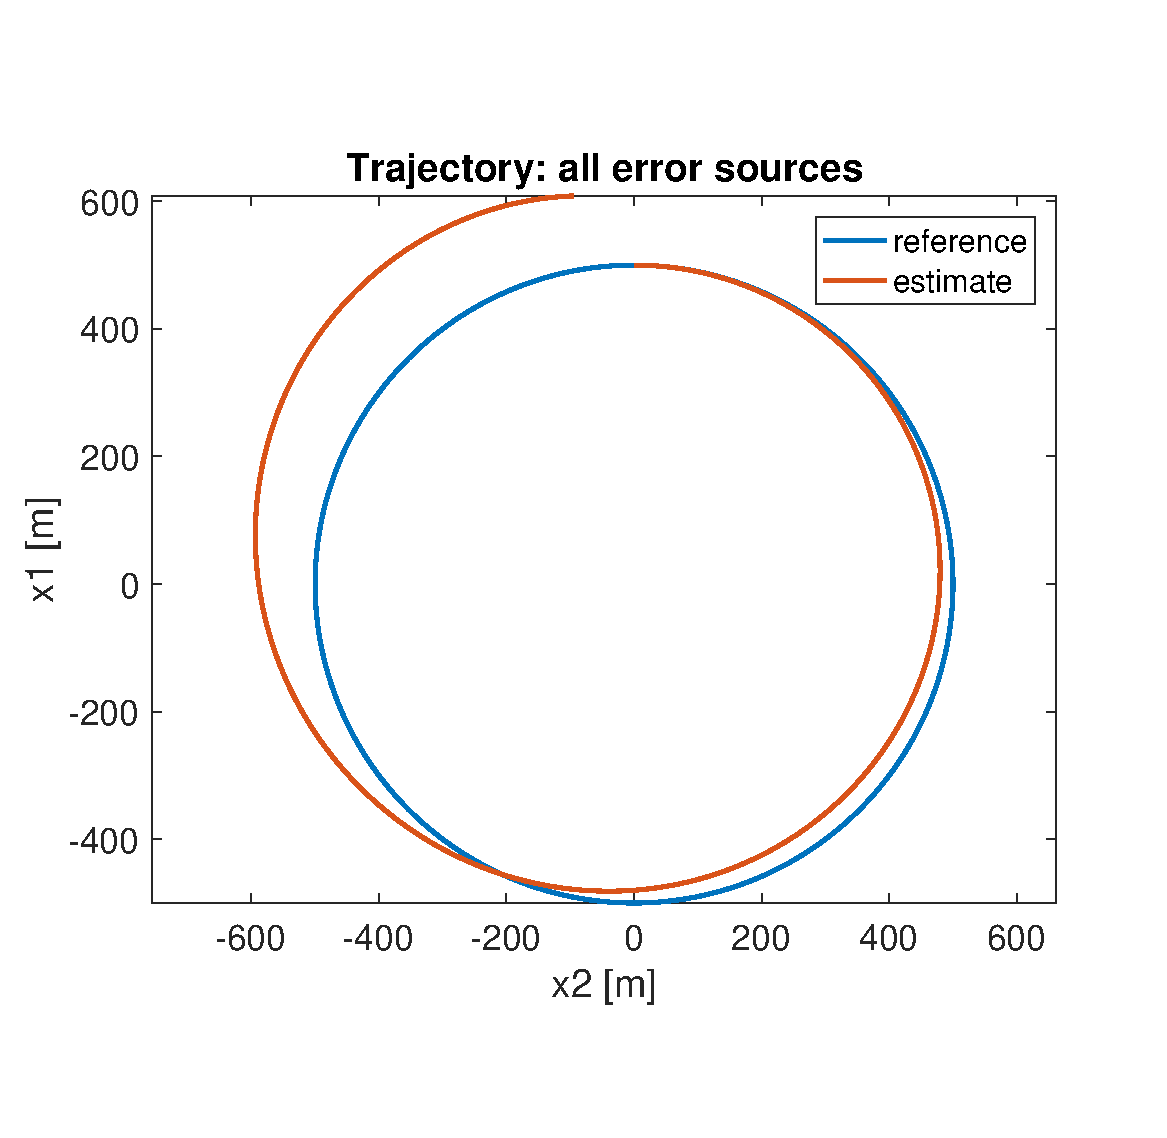
\includegraphics[width=\textwidth]{fig/traj_all}
        \caption{Estimate versus reference trajectory.}
    \end{subfigure}
    \caption{}
    \label{fig:error_all}
\end{figure}

\section*{Questions}

\subsubsection*{1) Which from the three error sources influences the \textit{least} the estimate of azimuth?}
The white noise resulted in the lowest error in the presented realization.
This is intuitive, since the noise mean is zero and integrating it for the azimuth
estimation should result in a lower error in comparison to noise with non-zero mean.
\\
Note: The Accelerometer errors are not considered, since it has no influence on the azimuth estimation.

\subsubsection*{2) Which error source influences the \textit{most} velocity estimation?}
The Accelerometer constant random bias resulted in the hightst velocity estimation error.

\subsubsection*{3) Which error source influences the \textit{most} position estimation?}
The Accelerometer constant random bias resulted in the hightst position estimation error.
This is intutive, since the acceleration is integrated twice for the position estimate, which means the position estimation error will not only grow but accelerate.

% \newpage
\section*{Code}
\lstinputlisting{../lab5.m}

\end{document}
